\chapter[Ensemble Modeling]{Ensemble Modeling}

\begin{objetivos}
By the end of this chapter, readers should understand ensemble SDM; integrate
GLM, GAM, Random Forest, BRT, and Maxent predictions; compare unweighted means,
performance-weighted means, and binary consensus; map ensemble suitability and
between-model agreement for \textit{Dinizia excelsa}; and prepare outputs for
future projections, uncertainty assessment, and conservation applications.
\end{objetivos}

\section{Introduction}

Ensemble modeling combines predictions from different algorithms rather than
depending on a single representation of the occurrence--environment relationship
\parencite{araujo2007ensemble,thuiller2009biomod,guisan2017habitat}. Algorithms
differ in response shape and flexibility: GLM and GAM are comparatively
interpretable, Random Forest and BRT capture complex structure, and Maxent is
designed for presence--background data. An ensemble summarizes this variation.

\begin{conceito}[title={\faBook\quad Ensembles in SDM}]
An ensemble combines multiple model predictions into an integrated suitability
estimate. It does not eliminate uncertainty; it makes agreement and disagreement
among algorithms explicit.
\end{conceito}

\section{Types of Ensemble}
\begin{itemize}
  \item unweighted mean prediction;
  \item mean weighted by predictive performance; and
  \item binary consensus based on presence--absence thresholds.
\end{itemize}
The unweighted mean assigns equal influence. A weighted mean favors models with
stronger evaluation scores. Binary consensus is the proportion of models that
classify a cell as suitable.

\begin{atencao}[title={\faExclamationTriangle\quad An ensemble does not repair a poor model}]
Only models meeting defensible quality criteria should enter the ensemble.
Including severely overfitted, low-quality, or ecologically incoherent models
can degrade the synthesis.
\end{atencao}

\section{Preparing Predictions}
The suitability rasters from Chapters 6--10 must share extent, resolution,
projection, and spatial mask.
\rscriptfile{scripts/unidade11/01_estrutura_pastas.R}
\rscriptfile{scripts/unidade11/02_preparar_predicoes_ensemble.R}

\section{Unweighted Mean Ensemble}
An unweighted mean is transparent and useful when component models have similar
performance.
\rscriptfile{scripts/unidade11/03_ensemble_media_simples.R}
\begin{figure}[H]
\centering
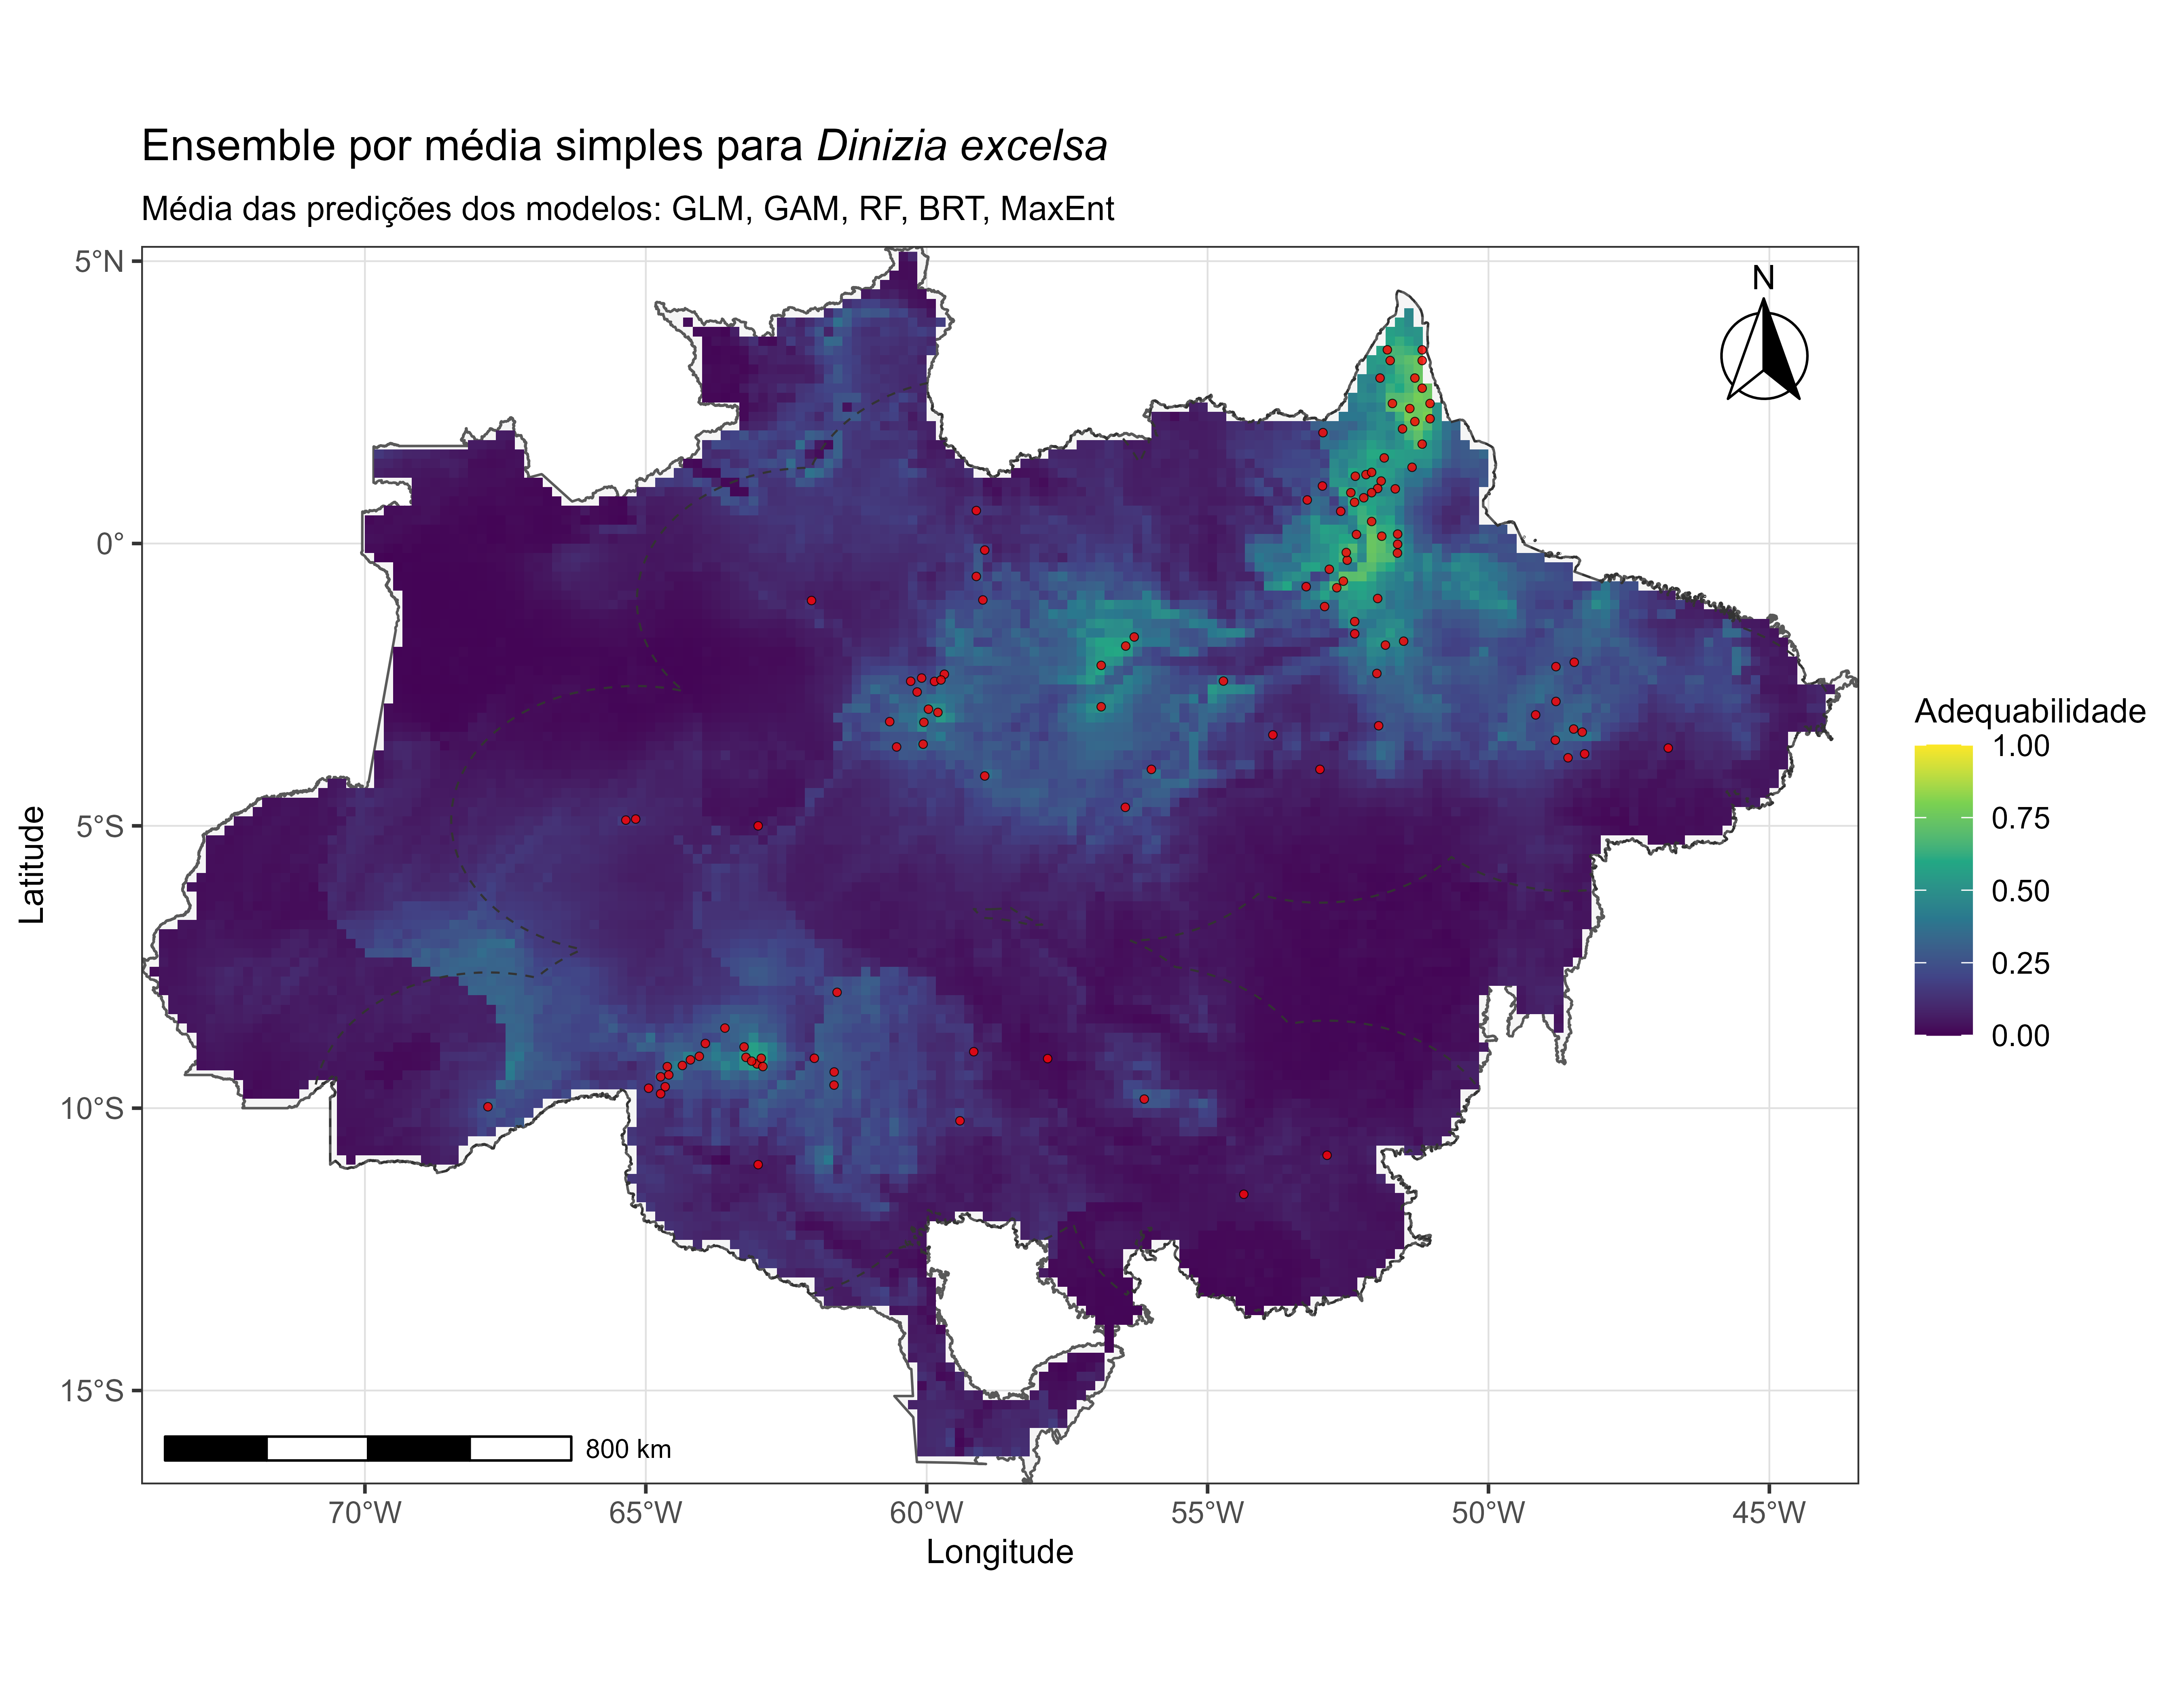
\includegraphics[width=0.88\textwidth]{figuras/unidade11/unidade11_ensemble_media_simples.png}
\caption{Unweighted mean of GLM, GAM, Random Forest, BRT, and Maxent predictions for \textit{Dinizia excelsa}.}
\label{fig:unidade11_ensemble_media}
\end{figure}

\section{Performance-Weighted Ensemble}
A weighted ensemble assigns greater influence to models with stronger
performance. Test AUC is used here, although TSS, Boyce Index, or a composite
criterion could be substituted. Weights inherit the strengths and limitations
of the selected metric and validation design.
\rscriptfile{scripts/unidade11/04_ensemble_ponderado.R}
\begin{figure}[H]
\centering
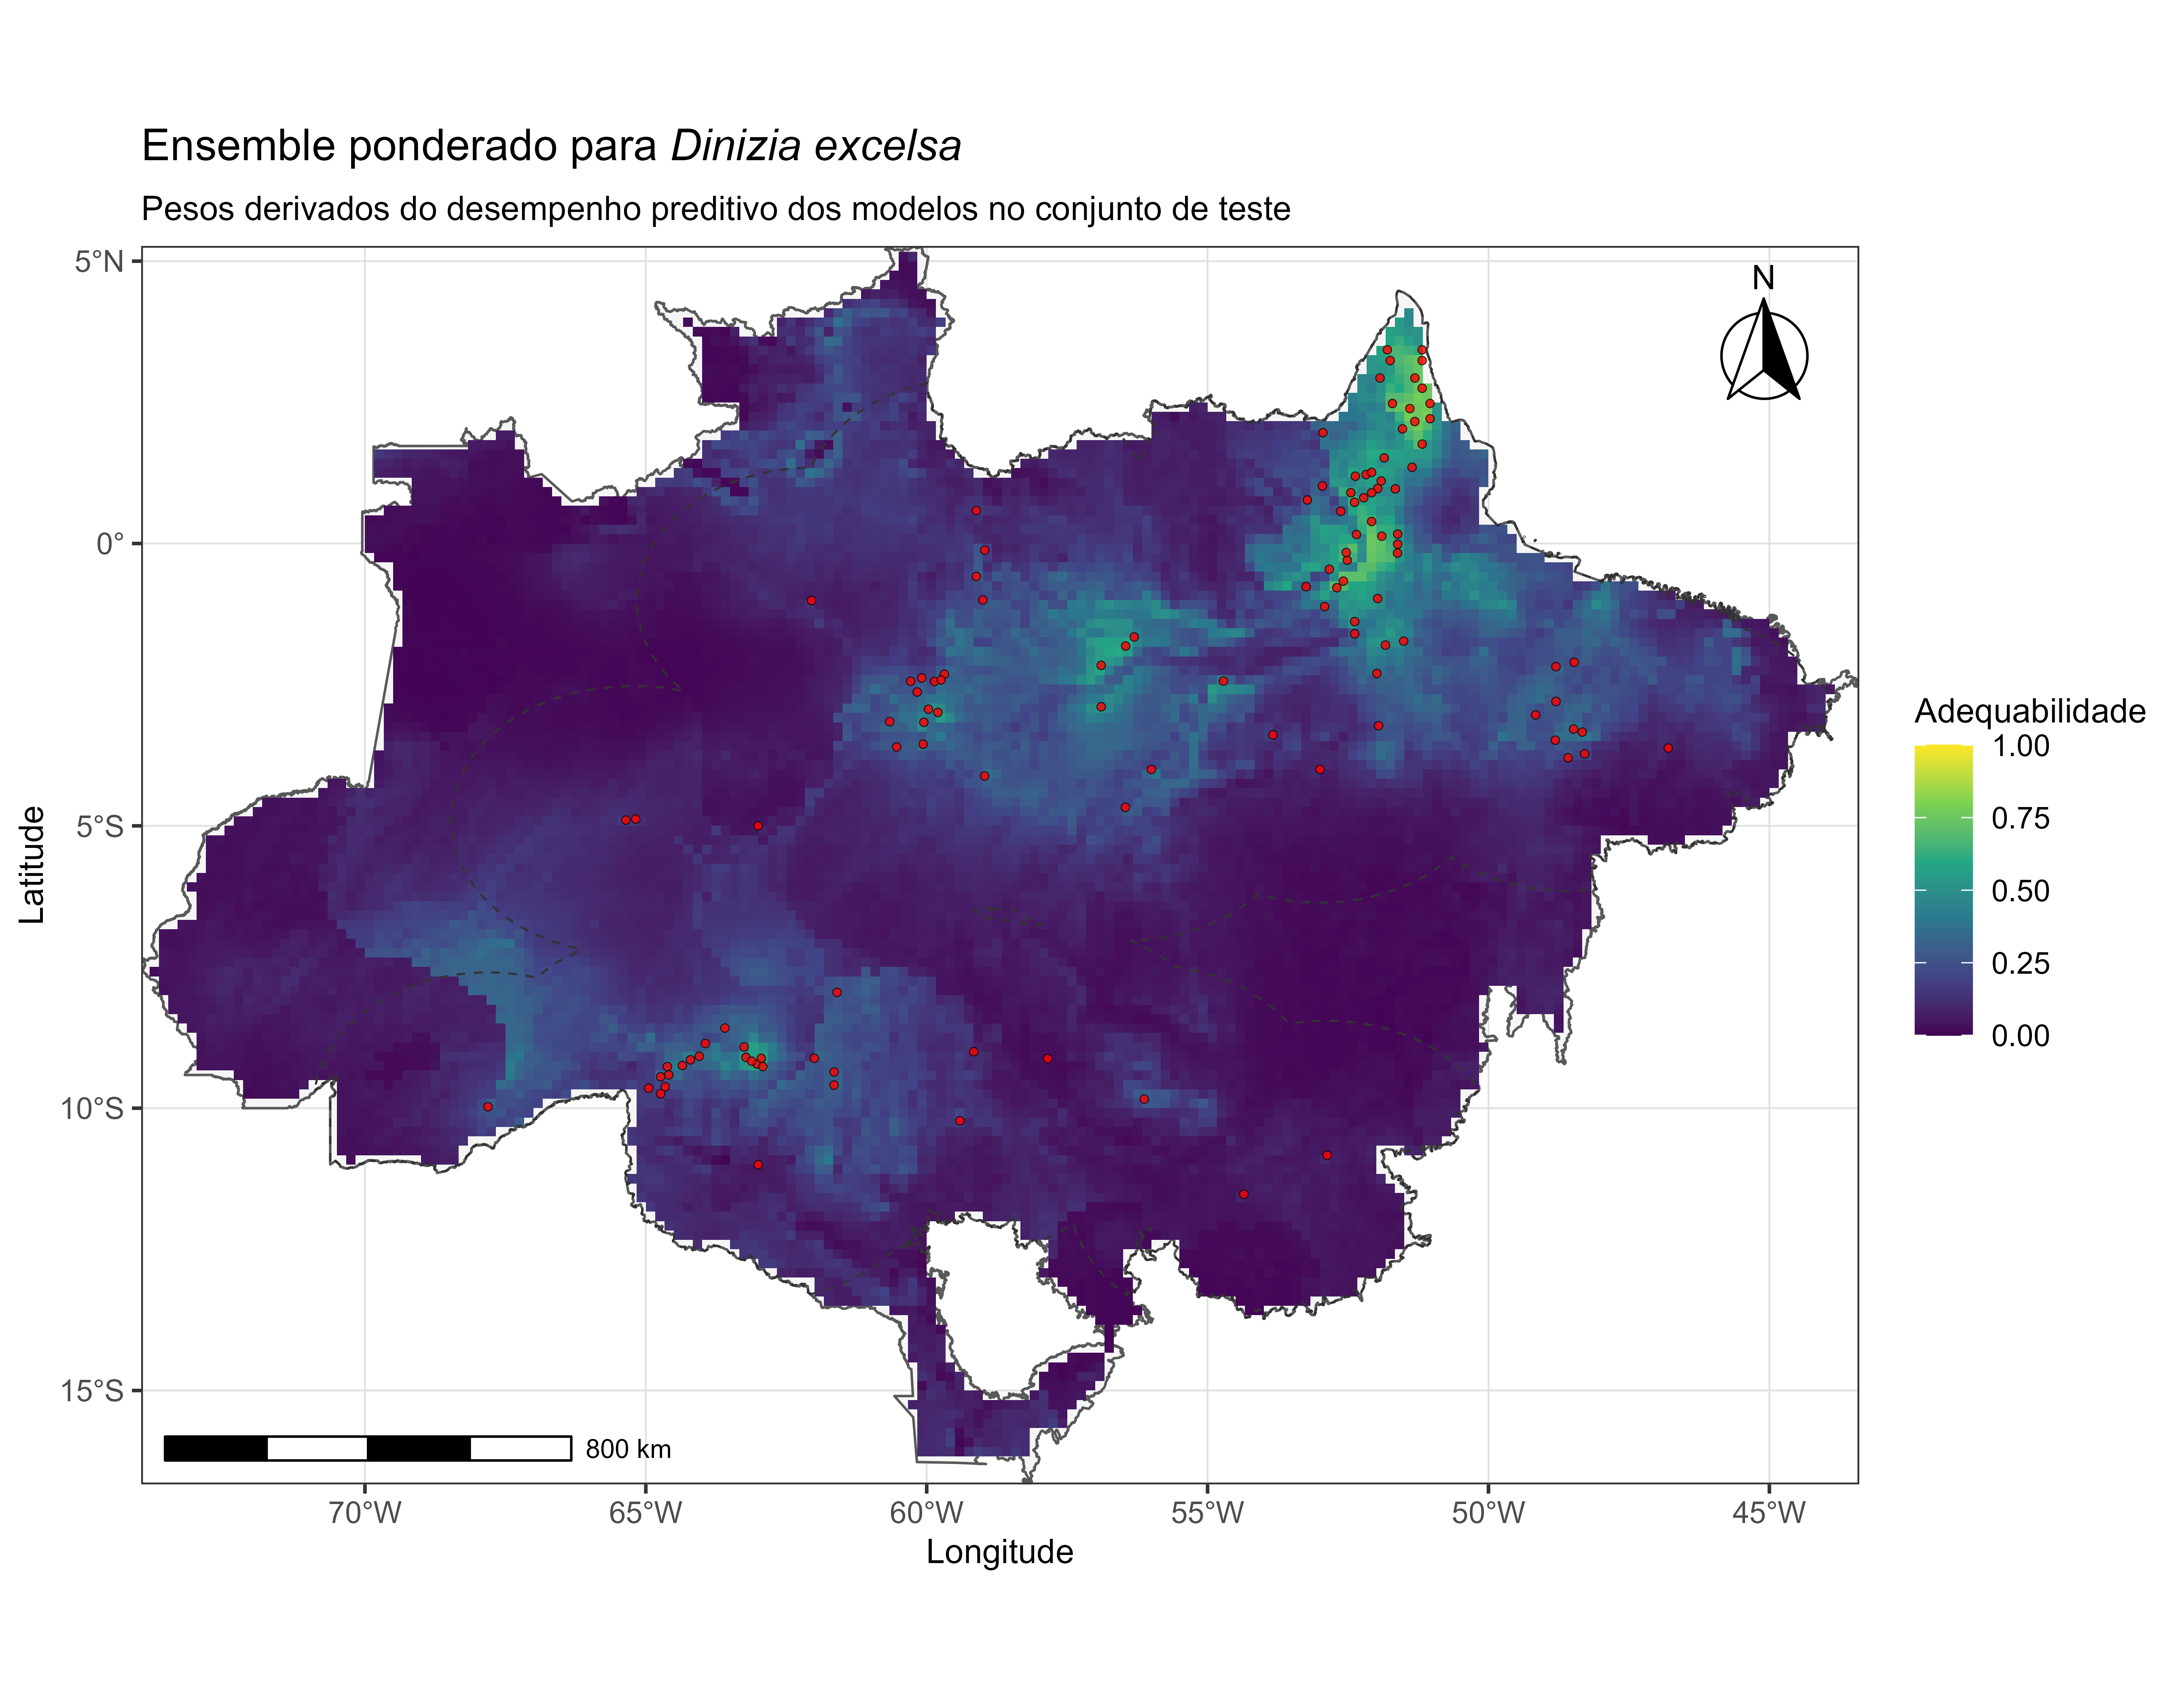
\includegraphics[width=0.88\textwidth]{figuras/unidade11/unidade11_ensemble_ponderado.png}
\caption{Performance-weighted ensemble suitability for \textit{Dinizia excelsa}.}
\label{fig:unidade11_ensemble_ponderado}
\end{figure}

\section{Binary Consensus}
Each continuous map is converted using its TSS threshold. The final value is the
proportion of models classifying a cell as suitable.
\rscriptfile{scripts/unidade11/05_consenso_binario.R}
\begin{figure}[H]
\centering
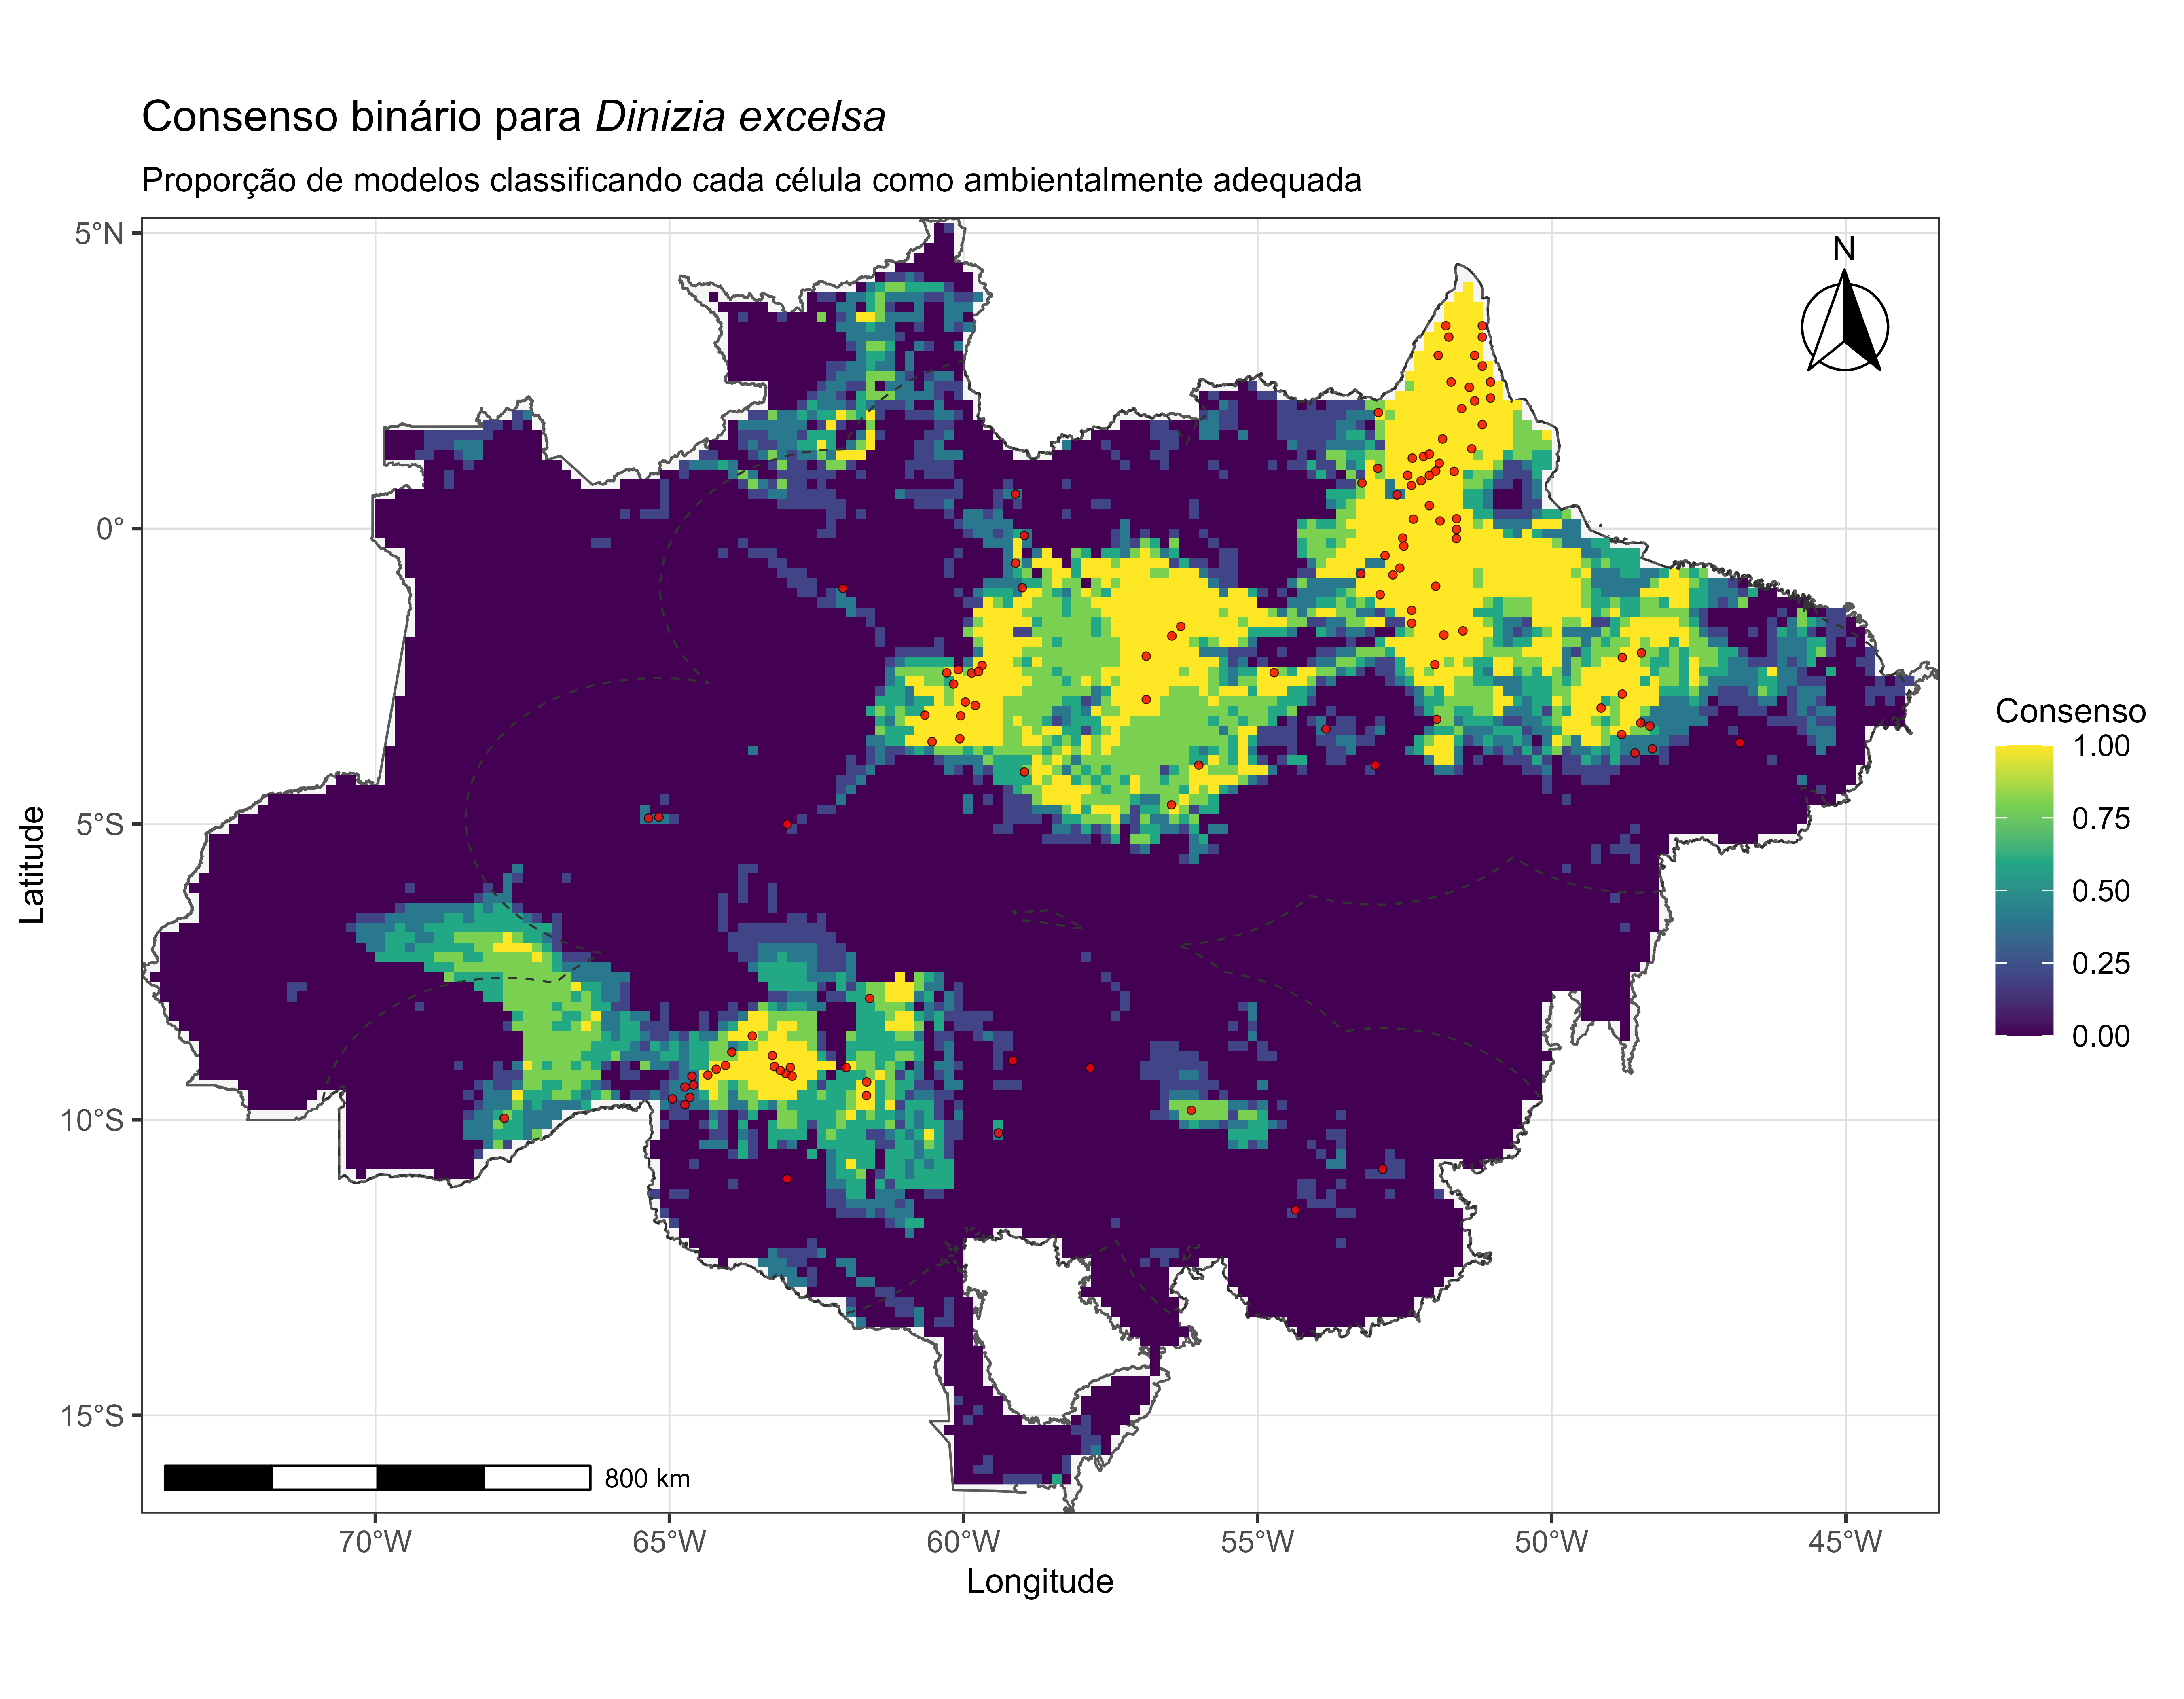
\includegraphics[width=0.88\textwidth]{figuras/unidade11/unidade11_consenso_binario.png}
\caption{Binary model consensus. Values near 1 indicate strong agreement that a cell is environmentally suitable.}
\label{fig:unidade11_consenso_binario}
\end{figure}

\section{Between-Algorithm Disagreement}
Variation among predictions is a descriptive measure of algorithmic disagreement. High mean
suitability with low variation is more robust than high suitability accompanied
by substantial model disagreement.
\rscriptfile{scripts/unidade11/06_incerteza_algoritmica.R}
\begin{figure}[H]
\centering
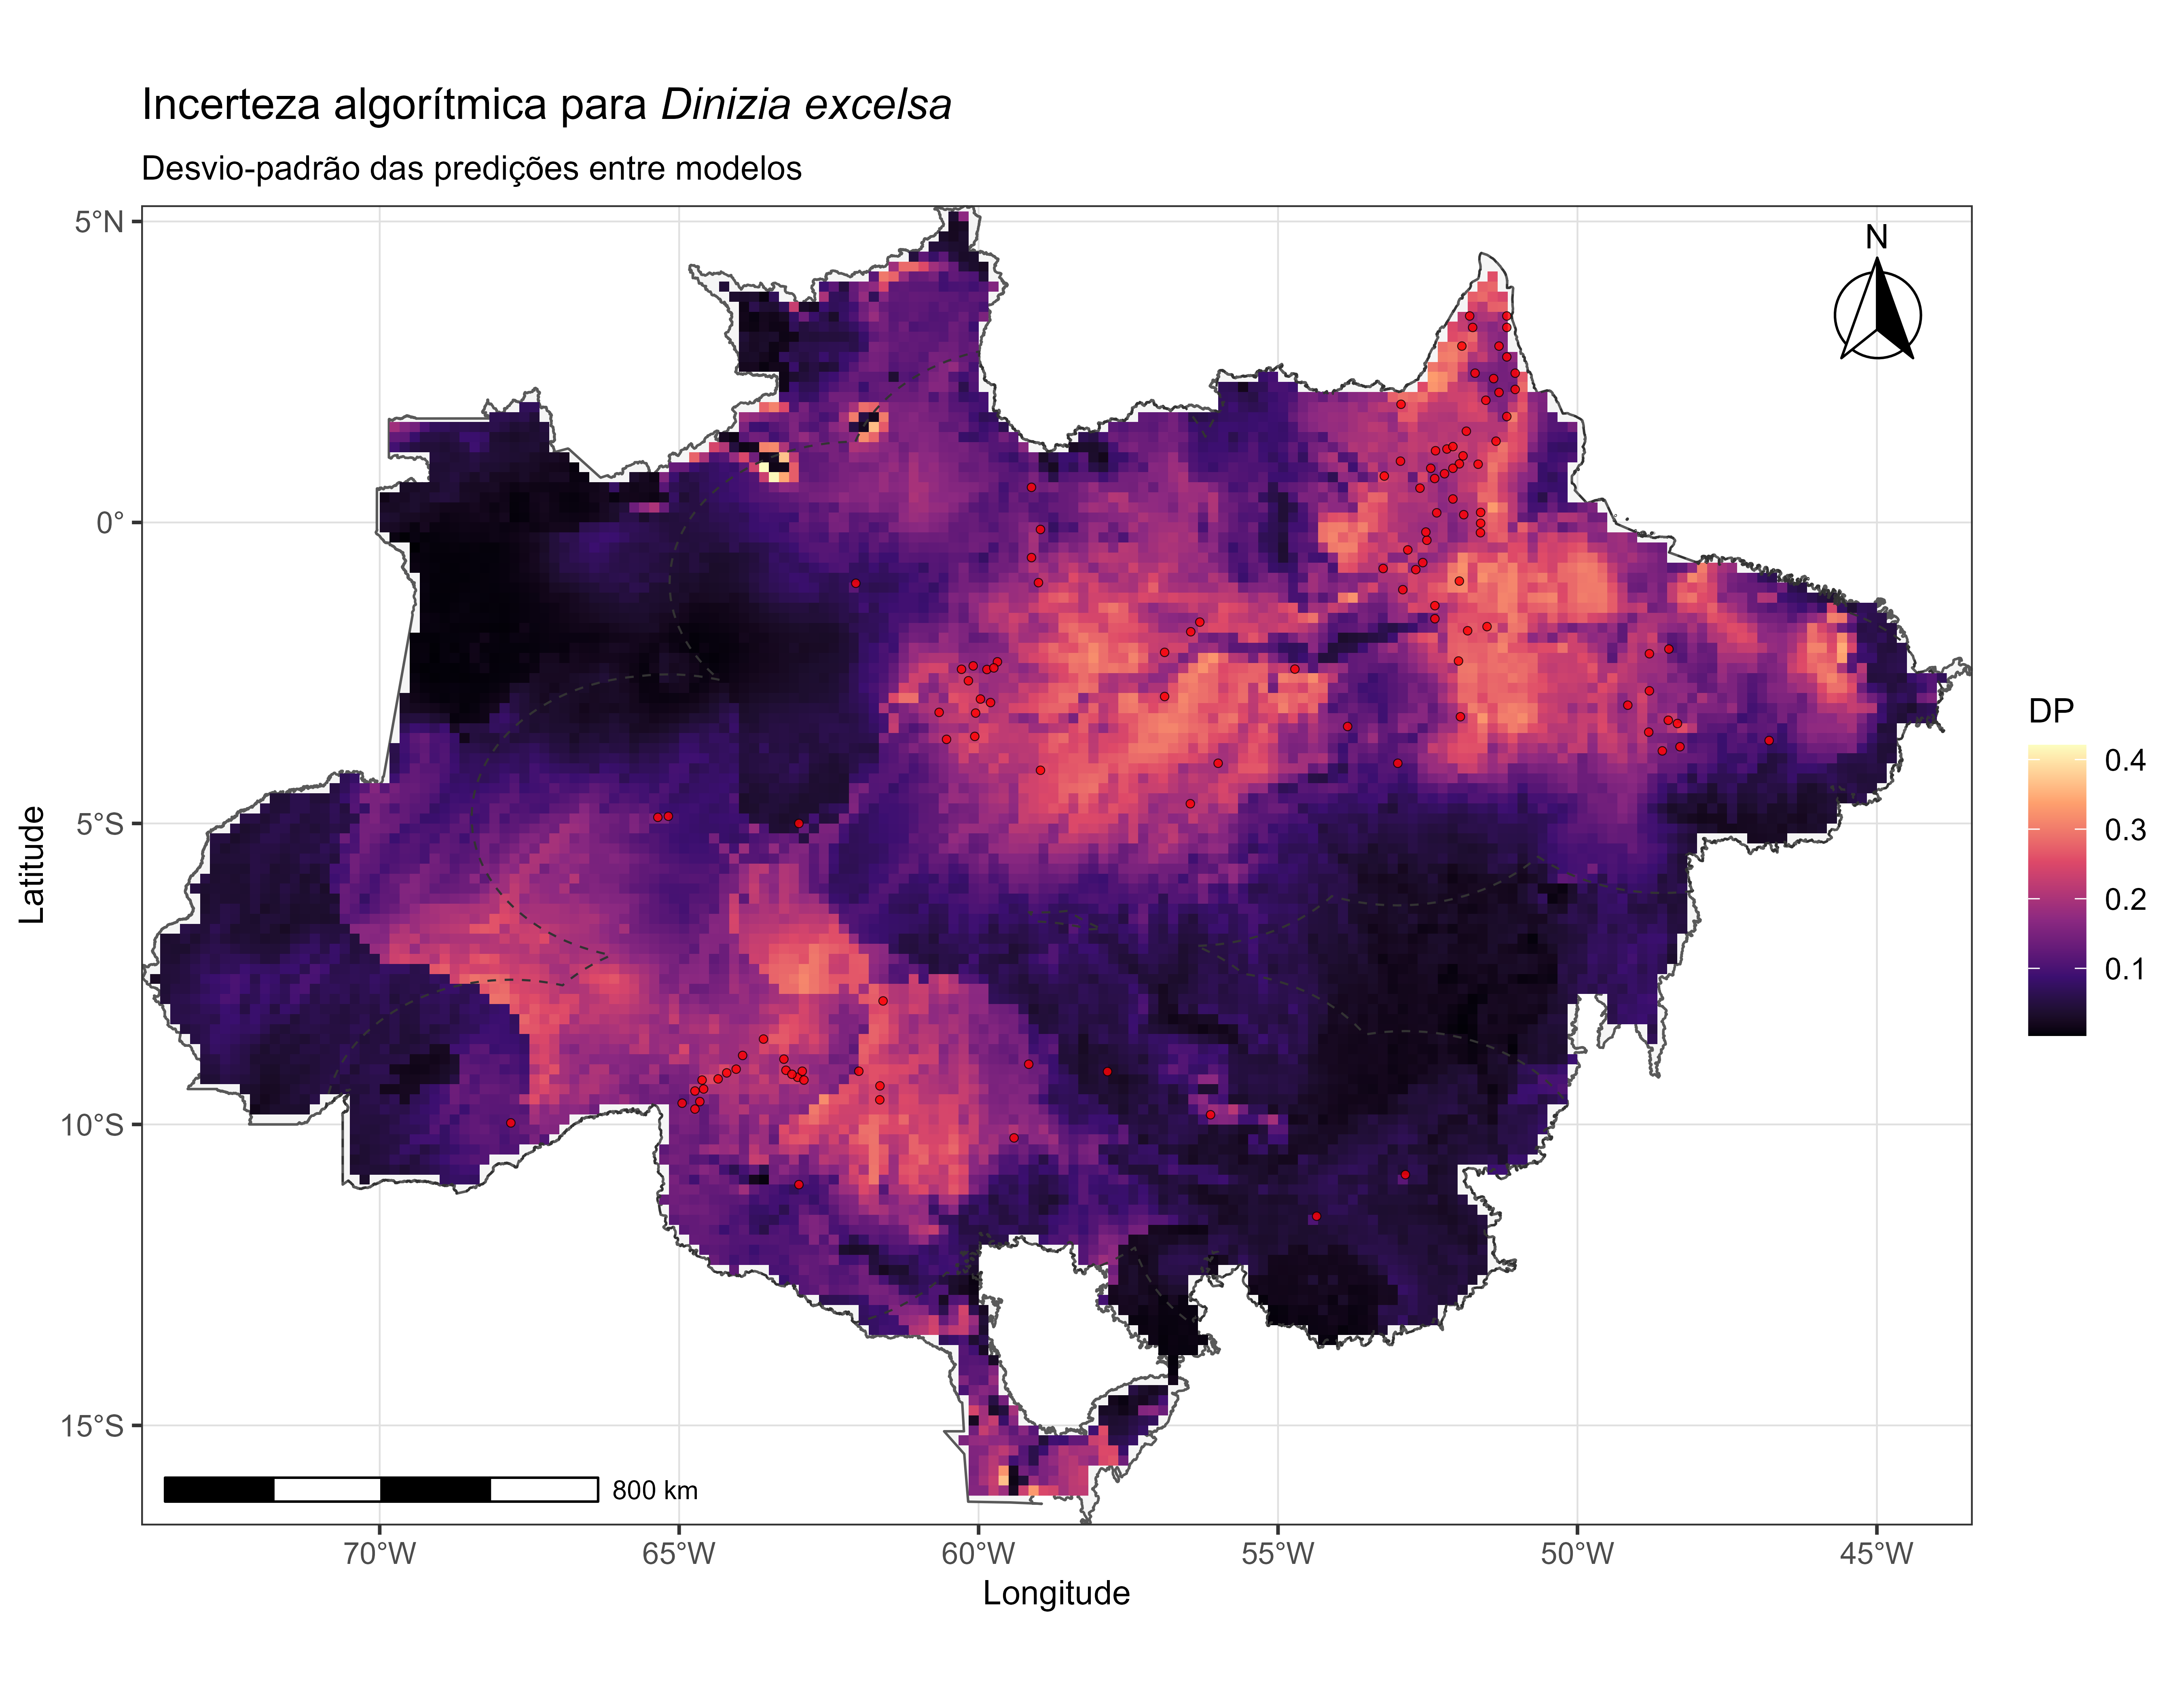
\includegraphics[width=0.88\textwidth]{figuras/unidade11/unidade11_incerteza_algoritmica.png}
\caption{Algorithmic disagreement summarized as the standard deviation among model predictions.}
\label{fig:unidade11_incerteza_algoritmica}
\end{figure}

\section{Integrated Comparison}
\rscriptfile{scripts/unidade11/07_comparacao_ensemble_modelos.R}
\begin{figure}[H]
\centering
\includegraphics[width=0.98\textwidth]{figuras/unidade11/unidade11_comparacao_ensemble.png}
\caption{Comparison of individual models, unweighted and weighted ensembles, binary consensus, and algorithmic disagreement.}
\label{fig:unidade11_comparacao_ensemble}
\end{figure}

\section{Complete Pipeline}
\rscriptfile{scripts/unidade11/08_pipeline_ensemble.R}

\section{Chapter Summary}
For \textit{Dinizia excelsa}, the ensemble integrates interpretable statistical
models and flexible algorithms to summarize present potential suitability
within $M$.
\begin{conceito}[title={\faBook\quad Key message}]
An ensemble does not replace critical evaluation of its components. Interpret
it together with evaluation metrics, response curves, ecological coherence,
and disagreement maps.
\end{conceito}

\section{Review Exercises}
\begin{enumerate}
\item Why are ensembles used in SDM?
\item Distinguish unweighted mean, weighted mean, and binary consensus.
\item Why should poor models be excluded?
\item How can algorithmic disagreement be mapped?
\item Why does a weighted ensemble depend on the selected metric?
\item How should high suitability with strong algorithmic disagreement be interpreted?
\item How can ensembles support future climate projections?
\end{enumerate}
